\chapter{Avoiding Leaks: Correlated Lifetime Patterns}
\label{chapter:lifetime-implementation-strategies}

Typically, objects die soon after the point in time of their last use, once all
dominating references are removed or naturally go out of scope. For a great many
objects, the normal flow of method invocations results in local variables going
out of scope, which renders these objects reclaimable without any special effort
on your part. In the absence of memory leaks, and without any optimizations,
objects live and die according to this \emph{natural lifetime}, as discussed in
depth in \autoref{sec:natural-lifetime}. 

However, the built-in lifetime mechanisms, by relying on objects going out of
scope, are insufficient to implement the more complicated patterns.
Implementations of the correlated lifetime pattern, introduced in
\autoref{sec:correlated-lifetime-pattern}, are very prone to memory leaks. You
may need an object to survive for a period of time that is not bound to any one
method invocation, but rather to the lifetime of another object. The lifetime of
some objects are indeed correlated with an invocation, as in the case of objects
correlated with a phase or request, but even here there are difficulties.
Oftentimes, the invocation that marks the beginning of a request is in a part of
the code outside of your control, or is distant from the allocation site of the
objects that must go away when the request finishes. Implementations of the
time-space tradeoff pattern, introduced in
\autoref{sec:time-space-tradeoffs-pattern}, can be ineffective if they aren't
sized properly. They, too, can result in memory exhaustion, e.g. if a cache's key
misimplement equality, or if it is sized too large.

It is important to code according to practices that will assure that an object
dies when it should. The correlated lifetime and time-space tradeoff patterns are
the most difficult cases to get right, and so those most in need of rigorous
coding practices.

Implementing a correlated lifetime pattern in a way that does not result in
memory drag or memory leaks is difficult. There are four important cases:
annotations, sharing pools, listeners, and phase/request-scoped objects.

\section{Tools: Weak References and Weak Maps}
\paragraph{Weak References}
The constructor for a \class{WeakReference} takes an object as a parameter. The
resulting instance of \class{WeakReference} is said to \emph{weakly reference}
that other object. A weakly referenced object will be garbage collectable, or
not, independently of being referenced from the \class{WeakReference} object; the
weak reference provides a non-owning handle to another object. This is a
sometimes helpful combination, to be able to refer to the object, without
inhibiting it being reclaimed as it normally would. To tunnel through the level
of indirection introduced by the weak reference, you call its \code{get} method.
If this method returns \code{null}, then you know that the referenced object has
been reclaimed. \autoref{chapter:correlted-lifetimes} discusses how to leverage
this functionality for an alternative implementation of the correlated lifetime
pattern.

There are three issues that you must handle with care. First, even though the
weak reference itself does not prolong the lifetime of the referenced object,
once you call \code{get}, you now have a regular reference to that object. If
this reference is stored in a local variable, or in a field of another object, or
in a collection, then you have now altered its lifetime. Once normally
referenced, the underlying object now obeys the lifetime rules discussed earlier.
Second, you must be careful to avoid race conditions, such as:
\begin{shortlisting}
class A {
   WeakReference<B> b;
   
   B getB() {
      if (b.get() != null) {
         return b.get();
      } else {
         // perform any necessary cleanup
         // notify caller of b's reclamation
      }
   }
}
\end{shortlisting}
In that code, between the first call to \code{b.get()} and the second, the
underlying object may have been reclaimed. You must modify that code to call
\code{b.get()} only once, and stash the result in a local variable until
\code{getB} returns. Third, if you need to be informed that the underlying object
has been reclaimed, you must use the \emph{reference queue} mechanism, which will
be discussed shortly.

\paragraph{The WeakHashMap}
\index{WeakHashMap}
\label{sec:weakhashmap}

The standard library includes an important construct, the \class{WeakHashMap},
that is not only quite useful, but also hides most of the complexity of managing
reference queues. A weak hashmap is a map that only weakly references its keys.
When a key is reclaimed, the map evicts the corresponding entry. Behind the
scenes, it uses weak references and reference queues, but you needn't worry about
any of that. Your own code is not polluted by mention of \class{WeakReference}
and \class{ReferenceQueue}, nor of the polling complexities necessary to keep the
reference queue from overflowing with reclaimed keys.

\paragraph{The Danger of Diamonds}
\label{sec:strongweakdiamonds}

Using a construct such as \class{WeakHashMap} is not a guarantee of success. The
danger lies in there being another reference to the key that is not a weak
reference. If this strong reference comes from the key data structure itself,
then there is no problem. It is expected that, for the expected lifetime of an
entry, there will be a strong reference that comes from another data structure
--- this is the reference that you expect to keep the entry alive. The main
danger lies in a second strong reference emanating from the value data structure
of a key's entry in the map. If you insert values that strongly reference the
key, as illustrated in \autoref{fig:strongweakdiamonds} then the key will very
likely never be uniquely owned by the weak reference, even after the expected
strong reference is reclaimed.

\begin{figure}[h]   % NMM added [h] just to make formatting look good on 201007023, not necessary
\centering
	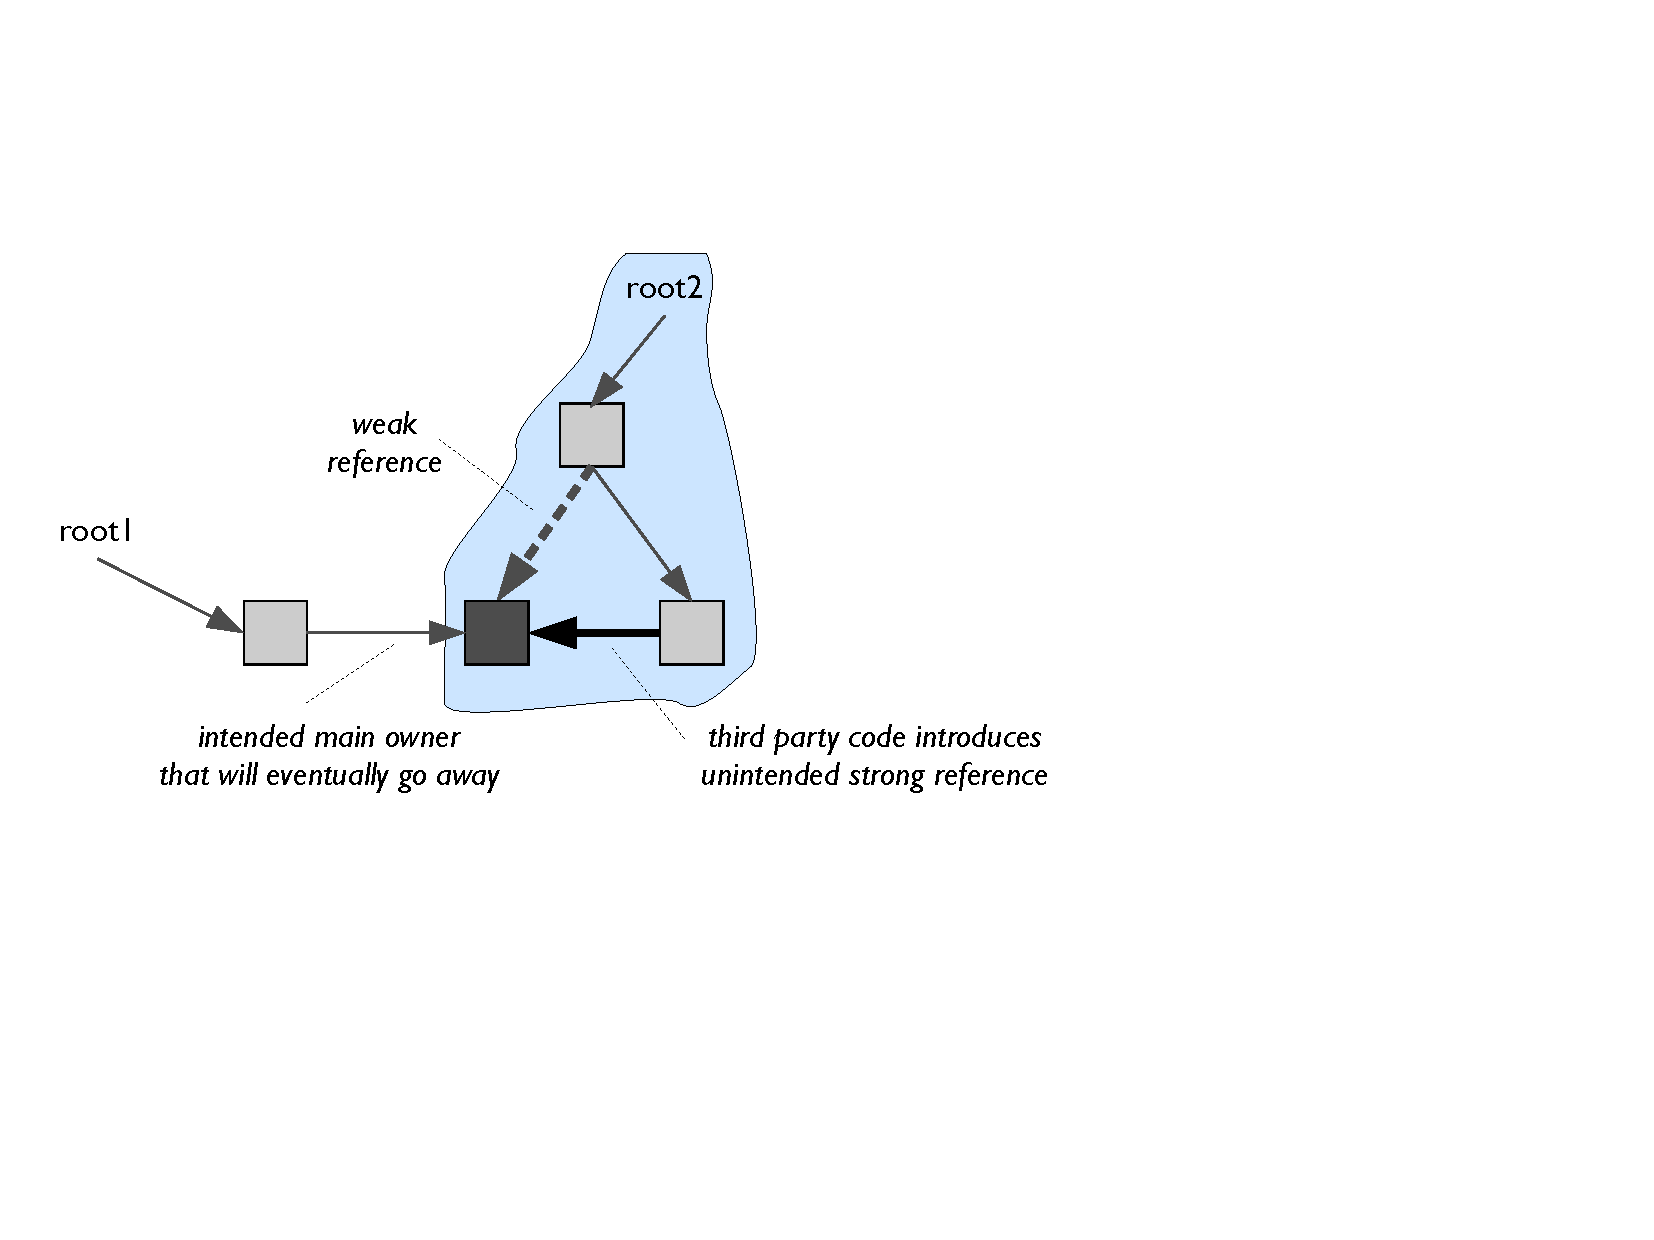
\includegraphics[width=0.6\textwidth]{part2/Figures/lifetime/strongweakdiamonds}
	\caption{Despite your best efforts to use weak references correctly, if you
	introduce a second strong reference in a way that forms a
	\emph{diamond} shape (the shaded region), it will likely never be reclaimed.}
	% [NMM] not sure if we need to give it a name, but, for now
	\label{fig:strongweakdiamonds}
\end{figure}

As is shown in the figure, this problematic reference structure has a diamond
shape. The top of the diamond is the \code{Entry} object of the map, from which
emanate two paths to the key, the weak reference from the \code{Entry} to the
key, and the strong reference path that flows through the value. In
\autoref{fig:strongweakdiamonds}, the darkly shaded object has a good chance of
never being reclaimed. 

In the following code, if \code{loopback} is true, then the \code{Finalized}
message will never appear.
\begin{shortlisting}
static public Object setupCycle(boolean loopback) {
   class Cycle {
       Object loopback;
   }
   class Entry {
       Object key;
       Cycle value;
   }
   Object key = new Object() {
           protected void finalize() {
               System.out.println("Finalized");
           }
       };
   Entry e = new Entry();
   e.key = new WeakReference(key);
   e.value = new Cycle();
   if (loopback) e.value.loopback = key;
   return e;
}
\end{shortlisting}

\section{Annotations}

If you don't have the luxury to change a class definition, but need to associate
some information with it, then your only choice is to use a map. To ensure that
the lifetime of the annotation is correlated with the lifetime of the annotated
object, you can use a \class{WeakHashMap}. \autoref{sec:weakhashmap} introduced
this utility class, that is part of the standard library. For example, to
associate a class \class{A} with a class \class{T}:

\begin{shortlisting}
class AnnotationMap<T,A> extends WeakHashMap<T, A> {
   public void annotate(T t, A a) {
      super.put(t, a);
   }
}
\end{shortlisting}

This implementation works well, at least for single-threaded programs. Soon after
an annotated T instance is reclaimed, the \class{WeakHashMap} will automatically
take care of removing the annotation entry from the map. If your application has
multiple threads concurrently accessing and creating these annotations, then you
will suffer from lock contention.
\autoref{sec:lifetime-management-concurrency-issues} discusses solutions to this
problem.

There is a more immediate potential problem, however. If your annotations are
more than simple objects like dates, then you have to be very careful to avoid
the strong-weak diamond problem described in \autoref{sec:strongweakdiamonds}.
This problematic situation can arise if an annotation, either directly or via
some chain of fields, strongly references the annotated object. This is a common
and innocent mistake, when you code in a way that avoids the messiness of
creating a reverse lookup map, from annotations to annotated objects:
\begin{shortlisting}
class TimestampAnnotation<T> {
   T t;
   Date date;
   
   public TimestampAnnotation(T t) {
      this.t = t;
      this.date = new Date();
   }
}
\end{shortlisting}
But this example will result in the annotation map leaking memory. You must have
the annotaitons weakly reference the annotated object, i.e. the \code{T t} field
must be replaced with a \code{WeakReference<T> t}. 
%Careful application of the
%single strong owner principle would help to avoid these mistakes. For example,
%you could offer a factory method 

%\begin{example}{Timestamp Annotation}
%How can you associate a timestamp with an object in a way that avoids memory
%leaks and that scales well to a highly concurrent workload?
%\end{example}
%
%We can start with the following code:
%
%\begin{shortlisting}
%class TimestampAnnotation<T> {
	%T t;
	%long timestamp;
%}
%List annotations;
%for (String string : inputList) {
	%...
	%annotations.add(new WeakReference(new Wrapper<String>(string)));
	%...
%}
%\end{shortlisting}
%
%Despite your use of \class{WeakReference}, you would find that neither the main
%object (the strings), nor the annotations, would ever be collected. This code
%has two memory leaks. One of the leaks is due to a
%violation of the first principal of the use of weak references: the annotations
%strongly reference the objects being annotated. It is not always this easy to
%debug problems in using weak references. Your application will hold on to
%objects that you didn't expect. Quite often, it is difficult to even know that
%there is a problem in the first place! The application may behave normally,
%except that it will consume more memory than necessary; if this extra memory
%consumption pushes it over your maximum heap size, then your application will
%crash --- you will know something is wrong, but diagnosing this type of
%problem, a memory leak\index{Memory Leak}, is quite difficult. It is better to
%keep the three principles of weak references in mind, and design in a way that
%avoids memory leaks in the first place. Your annotations can be modified to use
%a \class{WeakReference} to the main object:
%
%\begin{shortlisting}
%class TimestampAnnotation<T> {
	%WeakReference<T> t; // annotation only weakly refs main object
	%long timestamp;
%	
	%TimestampAnnotation(T t) {
		%this.t = new WeakReference(t);
	%}
%}
%\end{shortlisting}
%
%In this case, the annotation has no normal references to the annotated object,
%and so it obides by the first rule of weak references. If you remember from
%\autoref{chapter:delegation}, the code can be improved further to avoid the
%cost of delegation. This version of the annotation class extends
%\class{WeakReference}:
%
%\begin{shortlisting}
%class TimestampAnnotation<T> extends WeakReference<T> {
	%long timestamp;
%	
%	TimestampAnnotation(T t) {
		%super(t);
	%}
%}
%\end{shortlisting}
%
%Unfortunately, both of these updated versions h?
%%%%%%%
% old version??
%You could store the annotations in a map that is keyed by the
%original object, say of type \class{T}:
%
%\begin{shortlisting}
%Map<T, Date> timestamps = new HashMap<T, Date>();
%
%void addTimestamp(T t) {
	%timestamps.put(t, new Date());
%}
%Date getTimestamp(T t) {
%	return timestamps.get(t);
%}
%\end{shortlisting}
%
%This solution will function correctly, but suffers from a \emph{memory
%leak}\index{Memory Leak}. As the application runs, it will consume greater
%amounts of Java heap, up until the point when the \jre runs out of heap space
%to allocate any more objects. This solution leaks memory, because the
%\code{timestamps} map introduces a reference to the main objects. When the
%garbage collector scans the heap to see which objects are still alive, the
%references in this map will be among those that keep the objects alive. The
%next chapter discusses these issues in more detail. An improved solution would
%use the \class{WeakHashMap} from the Java standard libraries. By replacing the
%initialization of the \code{timestamps} map, we have the same functionality as
%before, but no memory leak.
%
%\begin{shortlisting}
%Map<T, Date> timestamps = new WeakHashMap<T, Date>();
%\end{shortlisting}
%
%Note that this same situation can hold even if you are able to modify the class
%definition. A common scenario requires annotations on only a subset of all
%instances of a class. In this case, is it not worth paying the memory cost to
%have the ability to annotate every single instance. Therefore, this is another
%case where a solution of side annotations, stored in a \class{WeakHashMap},
%shines.
%%%%%%%%%

\section{Sharing Immutable Data Safely}
\paragraph{Review of Sharing Pools}
\paragraph{A Leak-free Sharing Pool}
\paragraph{A Trickier Example: An Annotation Pool}
For the second requirement, Java provides some support for releasing unused
items from collections, namely, \class{WeakReference}s and \class{WeakHashMap}s. 
A \class{WeakReference} is an object wrapper. An object that is referenced by
a \class{WeakReference} can be reclaimed by the garbage
collector if there are no other strong references to it. A \class{WeakHashMap}
is a hashmap that stores keys as \class{WeakReferences}. That is, when there are no
strong references to a key, the entire entry is freed for garbage collection. 
 For example, we want an \class{Annotation} to
go away when its associated \class{Node}s are no longer used.
This can be implemented by a \class{WeakHashMap}:
\begin{shortlisting}
   WeakHashMap<Node><Annotation> nodeAnnotations;        (2)
\end{shortlisting}

This looks close to what we need. So let's modify (1) to be a
\class{WeakHashMap}, so that when an \class{Annotation} is no longer used,
 its sharing pool entry is freed for
garbage collection:
\begin{shortlisting}
   WeakHashMap<Annotation><Annotation> sharingPool;     
\end{shortlisting}
This should do it. Wrong! Both the key and the value of the sharingPool
 reference the same \class{Annotation} object. The key is a
weak reference, but the value is a strong reference, which prevents an
\class{Annotation} object from every being released. The value must also be a
\class{WeakReference}. Here is the correct
implementation of a sharing pool for \class{Annnotation}s:
\begin{shortlisting}
class AnnotationFactory {
   static WeakHashMap<Annotation, WeakReference<Annotation>>sharingPool = 
                   new WeakHashMap<Annotation, WeakReference<Annotation>>();
    
    public Annotation getAnnotation(Annotation annotation) {
        if (annotation == null) return null;
        WeakReference<Annotation> wref = sharingPool.get(annotation);
        if (wref != null) {
            Annotation oldAnnotation = wref.get();
            if (oldAnnotation != null) {
                return oldAnnotation;
            }
        }
        sharingPool.put(annotation, new WeakReference(annotation));
        return annotation;
    }
    ..
}
\end{shortlisting}

As this example shows,  Java's weak referencing capability has subtle
semantics and is not easy to use. Weak referencing is a lifetime management
facility, and is discussed in greater detail in Chapter~\ref{??} .


\section{Cleaning Up: Listeners}

Another common instance of the correlated lifetime pattern that is easy to mess
up is the listener pattern. A common implementation strategy is to have the list
of listeners be a list of strong references to the callback functions. The Java
Swing implementation of \class{JComponent} stores an \class{EventListenerList}
instance, which has an array of strong references to the callback handlers. This
implementation strategy has the benefit of being uniform: independent of whether
the listener list, or some other collection, is the home base for the callbacks,
you follow the same approach. Unfortunately, this approach requires that you
maintain and debug code that explicitly deregisters the callback hook from the
listener queue.

To avoid this source of bugs, you must follow the single strong owner principle.
You must choose which of the listener list or some other collection is the home
base for the callbacks. For example, if you already have a place to store the
callbacks, then the listener list can be created by a call to that home base
factory: {ListenerList list = factory.newList()}.  

\section{Phase/Request-Scoped Objects}

It is a huge challenge to ensure that an object created within a phase or request
dies soon after the phase or request completes. If the object is created at the
top level of the request method, and is never stashed into any static fields or
fields of objects which are bound to enclosing method scopes, then the normal
local variable scoping rules (see \autoref{sec:lifetime-of-locals}) would apply,
and life would be pretty easy:
\begin{shortlisting}
void doLogin() {
   Object obj = new Object();
   restOfWork(obj); // if obj does not escape ...
} // ... then lifetime of obj automatically ends here
\end{shortlisting}
If, during the execution of the \code{restOfWork} method,  \code{obj} does not
escape into some other scope, then its lifetime ends when the \code{doLogin}
method returns; and, possibly, somewhat before that, as discussed in
\autoref{sec:lifetime-of-locals}. The lifetime of the
object \code{obj} will be correlated with the \code{doLogin} request, by the
natural local variable scoping rules. However, it is very easy to write code that
alters the lifetime of \code{obj}. This is especially true if you have a
distributed team that are collaborating to implement the functionality of
\code{restOfWork}. Since the requirement, that the lifetime of \code{obj} be
correlated with the \code{doLogin} request is not specified in the code itself,
and likely not even in comments or documentation, the team does not know to
maintain this lifetime property. For example, a developer may choose to use
\code{obj} as the key into a longer-lived map. This is a common scenario, such
as when \code{obj} is a session identifier that is unique to the user's session
or to the specific request being processed. For example, if you are producing a
page composed of many parts, each part generated by independently written pieces
of code, you can glue them together via a \code{requestState} map:
\begin{shortlisting}
static Map requestState = new HashMap();
void restOfWork(Object requestKey) {
   requestState.put(requestKey, ...);
}
\end{shortlisting}
Now, these instances of \code{obj} will survive for an indefinite period of
time. There is no way to be sure of how long these keys will last, because it
ends on whether any of the \code{obj} intances are equal. If two calls to
\code{restOfWork} are passed equal objects, then the first one will be
reclaimable shortly after its entry in the map is replaced with the new one. 

It is also pretty easy to introduce a memory leak.\index{Memory Leak} If you
stash the object, in this case as a key, into a map, you must plan out a way to
remove it when the \code{doLogin} request is done. One solution is to associate a
cleanup hook with every data structure that should be correlated with a request,
and invoke these at the end of a request. You could use the Listener lifetime
pattern to do this. Each data structure that possibly contains request-scoped
objects must register as a listener. Then, assuming that the request is processed
by a single thread, you could combine the Listener lifetime pattern with a use of
\tls:
\begin{shortlisting}
/* the cleanup API */
interface CleanupHook { ... };

/* every thread keeps a registry of cleanup hooks */
static ThreadLocal<ListenerRegistry<CleanupHook>> requestLocals = new ThreadLocal<ListenerRegistry<CleanupHook>>() {
   public ListenerRegistry<CleanupHook> initialValue() {
      return new ListenerRegistry<CleanupHook>();
   }
}
void doLogin() {
   Object obj = new Object();
   restOfWork(obj); // obj might escape!
   requestLocals.get().notifyAll();
}
\end{shortlisting}

In some cases, this strategy can be made to work. Mostly, though, and even in the
current example, it is not a good approach. The \code{requestState} map is
global, used across all requests. How can you implement a \code{CleanupHook} that
knows which map entries to remove? In general, every data structure in which some
request-scoped objects are stored may have this problem. Each may have a
different requirement for extracting the correct objects, those for the request
that just completed, from the tangle that comes from many other concurrent
requests.

%Also, if your request spans multiple threads, then the above implementation
%simply won't work, because it relies on \tls. Support for
%multiple threads per request that is along the same lines would require
%keepoing track of those threads that participated. It would be pretty
%complicated to get the details working correctly, and maintain them.

How can you design a foolproof strategy that is minimally invasive? It would be
nice to piggyback on the automated reclamation that either local variable
scoping, or weak references offer. A single strong owner factory pattern, where
either a local variable of the top-most method in the request, or \tls, holds the
single strong reference to any request-scoped data:
\begin{shortlisting}
HomeBaseFactory requestLocals = new ThreadLocal_HomeBaseFactory();
void doLogin() {
   HomeBase myLocals = requestLocals.newOwner();
   Object obj = new Object();
   restOfWork(obj);
   // when myLocals goes out of scope, all request scoped objects will automatically become reclaimable
}
static Map requestState = requestLocals.newMap();
void restOfWork(Object requestKey) {
   requestState.put(requestKey, ...);
}
\end{shortlisting}

This implementation avoids the need for you to code any cleanup logic in the maps
and sets that store request-scoped data. You only need to alter the
\emph{constructor} of these maps to use the single strong owner pattern; as long
as you make sure to call \code{requestLocals.set(null)}, then any request-scoped
objects will be reclaimable immediately after the request completes --- all using
the normal, built-in scoping rules. It would be even better if you could arrange
it so that the \class{HomeBaseFactory} is a local variable of the
top-level request method; then, you only need to change the constructors of the
maps and sets that store request-scoped data. There are many minor variations of
this base implementation. You can tailor them to your specific needs.

\section{Cleaning up associated resources}
\paragraph{Finalizers and phantom references}
Java provides two other closely related cleanup hooks, in the form of
finalization and phantom references. These hooks are called just after the
garbage collector has discovered that the object is collectible, but before its
memory is reclaimed. If you implement a \code{finalize()} method in a class, then
every instance of that class will go through a finalization process. After being
discovered to be garbage, these instances will be enqueued on a special queue,
usually termed the \emph{finalizer queue}. Most \jres spawn a single thread,
termed the finalizer thread, that periodically scans the finalizer queue,
invoking the \code{finalize} method on the enqueued objects.

Phantom references offer a somewhat more refined version of this pre-reclamation
hook. First, with phantom references, you can associate a cleanup hook on a
per-object basis, rather than, as is the case with finalization, on a per-class
basis. Second, phantom references give you the option of having more than one
cleanup queue and thread, in contrast to finalization where there is a single
finalizer queue and (usually) a single finalizer thread.

You can use the hooks offered by finalization or phantom references to free up
resources that are implicitly associated with an object. Any Java objects
uniquely owned by this object will be reclaimed in the normal course of garbage
collection. It is those resources that are \emph{implicitly} tied to a Java
object, such as file descriptors, socket connections, and database resources such
as compiled queries, that require special attention.

You must be very careful in relying on finalization or phantom references. The
Java language specification provides no assurances of how often, or even whether,
finalization will be run on an object. In the normal course of program execution,
eventually the finalizer will run. This is because the finalizer queue consumes
Java heap, and hence the finalizer thread will always do whatever finalization is
possible before the \jre gives up due to heap exhaustion. However, if your Java
objects serve as proxies for some native, or remote, storage, and the space
consumed by the Java proxies is small compared to the external state, then you
may have problems. The \jre knows nothing about this external state, and so will
not schedule the finalizer thread if an external resource is exhausted.

Furthermore, the specification is very lax about whether finalizers will be run
before program termination. You can ask the \jre to attempt to finalize objects
before the program terminates, by calling
\code{System.runFinalizersOnExit(true)}, a deprecated part of the API. However,
most \jres these days run only a partial finalization, if you ask. It is hard for
the \jre to do the right thing in a deadlock free manner. Should it only schedule
the finalizer thread, which would run any pending finalization? This would be
safe, and is what the \jre will do if you ask. But this misses all the
currently-live objects that would have have been finalized, had the program
reached a point where they were reclaimable. The \jre can't unwind, on exit, all
the Java references thta keep those objects alive. Also, there is no analogous
request to have the \jre run a garbage collection on exit. Hence, even for those
objects which are actually ready to be finalized, the \jre won't do so on exit.
It is for these reasons that the API has been deprecated.

Given these downsides, it is best for you to implement a more robust lifetime
management strategy. If you can establish a correlated lifetime pattern, such as
that the external storage should be reclaimed when an event occurs, or when a
method returns, then you should do so.

\section{The Single Strong Owner Pattern}

Lifetime management for temporaries (the lifetime pattern discussed in
\autoref{sec:temporary-lifetime}), and for objects that are part of only one data
structure at a time is usually pretty straightforward. The lifetime of a
temporary object, such as one created within a method and not used beyond the end
of the method, will be nicely governed by local variable scoping rules.

Many lifetime management bugs arise from shared ownership of non-temporary
objects. When an object that is simultaneously part of more than one data
structure, as introduced in \autoref{sec:shared-ownership}, it becomes hard to
keep track of what actions need to be taken in order to make that object
reclaimable by the \jre. Even if you make your best effort to avoid this problem,
such as by using weak references, you can still have problems. The diamond
structures described in \autoref{sec:strongweakdiamonds} are a good example of a
case where, even with weak references, objects may stick around too long. What
programming patterns can help to avoid these problems, so that you aren't left
hunting down hard to diagnose memory leaks late in the development lifecycle?

Ideally, every object would be part of only one data structure at a time. This
would simplify lifetime management issues, because there would be no hidden
links for you to track down and eliminate. This is of course not possible in any
practical setting. It is necessary for multiple, probably unrelated, parts of
the code to need access to a common set of objects. The listener pattern,
covered in more detail below, is a common case of this. For example, in user
interface code, both the callback handler for user events and the redraw loop
will operate on the underlying data model that the view exposes.

A more practical spin on this single-owner ideal is that every object
should have a \emph{home base}.
\callout{home-base}{The Home Base as Single Strong Owner}{
%A good design principle is to consider that every object, 
If an object simultaneously is part of
multiple data structures, then identify one of these as its \emph{home base}.
The home base data structure should be the \emph{single strong owner} of this
shared object. Every other data structure must only weakly or softly reference the
object.}

For example, consider an object that is part of a cache. While it is not in use,
the cache is the sole owner of the objects. If it weren't for the cache holding
a non-weak reference to the object, it would be reclaimed. When a cached object
is being used by the program, it will likely also be part of other data
structures; these structures may possibly span multiple threads. The cache is a
natural home base, and any other transitory owners of the objects msut be
designed so that their ownership is indeed transient.

A first piece of implementing this single strong owner pattern is the home base
itself:
\begin{shortlisting}
class HomeBase {   
   Set owned = new HashSet();
   
   public void own(Object o) {
      owned.add(o);
   }
}
\end{shortlisting}

%\lstset{moredelim=[is][\underbar]{|}{|}}

On its own, the \class{HomeBase} class provides a repository for strong
references, but doesn't help much in assuring that it is the \emph{only} strong
reference to the objects.To add this extra level of assurance requires four
pieces of logic. First, you need to make sure that every other collection in
which these objects are placed does not have a strong reference to the object.
Second, it would be a big headache to have to call
\class{HomeBase.own()} on every object that you create. This would
heavily pollute your code and be a nightmare to maintain. You can combine the
first two, if there are facades for the collections that take care of the
registration process for you. Third, there are several important use cases for
which the collections are intended to hold data for multiple tasks. Therefore,
you can't simply associate one \class{HomeBase} repository with a
collection; e.g. you may have a single map that contains data for multiple
tasks, each of which needs its own repository. The final issue is how to ensure
that the repository itself becomes reclaimable soon after you are done with it.
A rigorous coding practice is necessary to avoid holding on to the repository
itself for longer than necessary.

You can use a factory design pattern to help. The factory should have this basic
structure:
\begin{shortlisting}
class HomeBaseFactory {
   public HomeBase newOwner() {
      return new HomeBase();
   }

   public Map newMap(HomeBase home) {
      return new WeakHashMap() {
         public Object put(Object key, Object value) {
            home.own(key); return super.put(key, value);
         }
      }
   }
}
\end{shortlisting}
In this base implementation, the \code{newOwner} method doesn't do anything
fancy. But it does provide factory methods for creating a map facade that takes
care of associating ownership with a given repository, while keeping the map
itself free of eternally persistent references to the map's contents. Once the
repository is reclaimed, then the weakly referenced key will be reclaimed, at
which point, or shortly thereafter, the \class{WeakHashMap} will take care of
removing the entire entry (see \autoref{sec:weakhashmap}). From this base
implementation, it should be easy for you to implement similar factory methods
for the other kinds of collections, such as sets and lists.

It is often the case that the repository for ownership can reside within a
thread. If so, you can leverage the \tls mechanism to implement
a factory that provides unique ownership respositories
\begin{shortlisting}
class ThreadLocal_HomeBaseFactory extends HomeBaseFactory {
   ThreadLocal<HomeBase> threadLocals = new ThreadLocal<HomeBase>();
   
   protected void own(Object o) {
      // the thread's HomeBase assumes ownership
      return threadLocals.get().own();
   }

   public HomeBase newOwner() {
      HomeBase home = new HomeBase();
      threadLocals.set(home);
      return home;
      // the caller will now have the only strong reference to the HomeBase repository, we maintain only a weak reference to it
   }
}
\end{shortlisting}

But this implementation suffers from memory drag. After the thread's task
completes, the \tls maintains a reference to the \class{HomeBase} and
all the owned objects. It will only be overwritten either when the same thread is
scheduled to process a new task, or when the thread terminates. You could
overcome this by adding a \code{clear} method, and inserting a call to it at the
right place in your code:
\begin{shortlisting}
public void clear() {
   threadLocals.set(null);
}
\end{shortlisting}
However, this is a messy and error prone solution. An alternative solution is to
rely on local variable scoping to automatically clean things up for you. When a
task begins, you can grab a strong reference to the \class{HomeBase}
repository, and have the \tls maintain only a weak reference to
it:
\begin{shortlisting}
class ThreadLocal_HomeBaseFactory extends HomeBaseFactory {
   ThreadLocal<WeakReference<HomeBase>> threadLocals = new ThreadLocal<WeakReference<HomeBase>>();
      
   protected void own(Object o) {
      // the thread's HomeBase assumes ownership
      return threadLocals.get().get().own();
   }
   
   public HomeBase newOwner() {
      HomeBase home = new HomeBase();
      threadLocals.set(new WeakReference(home));
      return home;
      // the caller has the only strong reference to the HomeBase repository, we maintain only a weak reference to it
   }
}
\end{shortlisting}
Now, all objects owned by the repository will be automatically reclaimable when
the return value of \code{newOwner} goes out of scope.

\section{Summary}



